\chapter{Conexión}%
\label{cha:conexion}
\section{Concepto y mantras}%
\label{sec:concepto_y_mantras_conx}
\begin{defi}
$X$ es \underline{conexo} si cumple las siguientes condiciones equivalentes:
\begin{enumerate}
    %TODO: union rara
    \item $\nexists X = U \sqcup Y$ abiertos $\neq \emptyset$.
    \item $\nexists X = F \sqcup C$ cerrados $\neq \emptyset$.
    \item $\nexists E \subsetneq X$ abierto y cerrado $\neq \emptyset$.
\end{enumerate}
\end{defi}
\begin{demo}
Equivalencia: $F = X \setminus V,\ C = X \setminus U,\ E = U = X \setminus V.$
\end{demo}

\begin{obs}
$Y \subset X$ subespacio conexo: $\nexists Y \subset U \cup V$ abierto de $X$, 
\[
\begin{cases}
    U \cap Y \neq \emptyset\\
    V \cap Y \neq \emptyset\\
    U \cap V \cap Y = \emptyset
\end{cases} 
\]
\end{obs}

\begin{ej}[Fundamental]
$\left( 0, 1 \right) \subset \mathbb{R}_u$ es conexo. 

Mantras generales $\Rightarrow$ segmentos en $\mathbb{R}^n$, estrellados? y conexos son conexos.
\end{ej}

\begin{theo}[del pivote. Mantra 1] 
Sea $X = \bigcup_{i} A_i,\ \bigcap_{i} A_i \neq 0,\ \forall A_i$ conexos $\Rightarrow X$ conexos.
\end{theo}
\begin{demo}
\begin{align*}
    \emptyset \neq E \stackrel{\text{ab. cerr.}}{\subset} X &\Rightarrow \forall i,\ E \cap A_i \stackrel{\text{ab. cerr.}}{\subset} A_i \Rightarrow \forall i,\ \begin{cases}
        E \cap A_i = \emptyset\\
        E \supset A_i
    \end{cases}\\
    &\xRightarrow{E \neq \emptyset} \exists i_0: E \supset A_{i_0} \supset \bigcap_{i} A_i \neq \emptyset \Rightarrow \forall i,\ E \cap A_i \neq \emptyset \Rightarrow \forall i,\ E \supset A_i\\
    &\Rightarrow E \supset \bigcup_{i} A_i \Rightarrow E = X
.\end{align*}
\end{demo}

\begin{coro}[Variantes]
\begin{enumerate}
    \item $X = \bigcup_{i \in  I} A_i,\ \exists A_{i_0} \cap A_i \neq \emptyset$.
    \begin{demo}
        $X = \bigcup_{i \in  I}\left( A_{i_0} \cup A_i \right)$ conexo por mantra $1$ y se aplica el mantra $1$.
    \end{demo}
    \item Cadenas: $X = \underbrace{A_1 \cup \ldots \cup A_k \cup \ldots}_{\text{conexos}}\quad A_k \cap A_{k + 1} \neq \emptyset \Rightarrow X$ conexo.
    \begin{demo}
        Se usa el mantra $1$ dos veces:
        \[
        \begin{cases}
            X_k = \left( \ldots \left( \left( A_1 \cup A_2 \right) \cup A_3 \right) \cup \ldots \cup \right) A_k\\
            X = \bigcup_{k} \left( X_1 \cup \ldots \cup X_k \right) 
        \end{cases} 
        \]
        %TODO: Imagen
        \begin{center}
            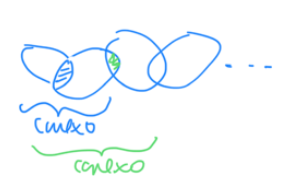
\includegraphics[scale=0.3]{images/dem_var_mantra_1_conx} 
        \end{center}
    \end{demo}
\end{enumerate} 
\end{coro}

El ``recíproco'' es ``fácil'' pero útil.
\begin{prop}[Construcción de cadenas]
$X$ conexo, $X = \bigcup_{i} U_i$ recubrimiento abierto, $p, q \in X \Rightarrow \exists$ cadena finita $U_{i_k}$ de $p$ a $q: p \in U_{i_0}, U_{i_{k - 1}} \cap U_{i_k} \neq \emptyset,\ q \in U_{i_r}$. 
\end{prop}
\begin{demo}
$A = \{x \in X: \exists U_{i_k} \text{ de } p \text{ a } x\} \neq \emptyset$ abierto y cerrado $\Rightarrow A = X$ y $q \in A$. Por ser:
\begin{itemize}
    \item $\neq \emptyset: \exists U_{i_0} \in? p$ y $U_{i_0}$ va de $p$ a $p$ !
    \item Abierto: $\exists U_{i_0}, \ldots, U_{i_r}$ de $p$ a $x \Rightarrow U_{i_r} \subset A$.
    \item Cerrado: 
    \begin{align*}
        y \in \overline{A} \text{ e } y \in U_{i\left( y \right)} &\Rightarrow A \cap U_{i\left( y \right)} \neq \emptyset\\
        &\Rightarrow \exists U_{i_0}, \ldots, U_{i_r} \text{ de } p \text{ a } x\in U_{i\left( y \right)}\\
        &\Rightarrow U_{i_0}, \ldots, U_{i_r}, U_{i\left( y \right)} \text{ de } p \text{ a } y
    .\end{align*}
\end{itemize}
%TODO: Imagen
\begin{center}
    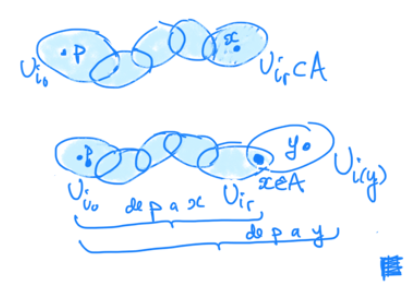
\includegraphics[scale=0.3]{images/dem_const_cadenas} 
\end{center}
\end{demo}

\begin{prop}[Mantra 2]
Imagen continua de conexo es conexo. 
\end{prop}
\begin{demo}
    $f: X \rightarrow Y$ continua, $\emptyset \neq E \stackrel{\text{ab. cerr.}}{\subset} f\left( X \right) \xRightarrow{\text{cont.}} \emptyset \neq f^{-1}\left( E \right) \stackrel{\text{ab. cerr.}}{\subset} X \Rightarrow f^{-1}\left( E \right) = X \Rightarrow E = f\left( X \right)$.
\end{demo}

\begin{prop}[Mantra 3]
Adherencia de conexo es conexo: $Y \subset X$ con $Y$ conexo y denso $\Rightarrow X$ conexo. 
\end{prop}
\begin{demo}
    $\emptyset \neq E \stackrel{\text{ab. cerr.}}{\subset} X \Rightarrow E \cap Y \stackrel{\text{ab. cerr.}}{\subset} Y \Rightarrow \begin{cases}
        E \cap Y = \emptyset\ \times \text{densidad.} \\
        E \cap Y = Y \Rightarrow Y \subset E \cerr X = \overline{Y} \Rightarrow E = X.
    \end{cases}$
\end{demo}

\begin{ej}
   %TODO: Ejemplos complicados
    \begin{enumerate}
        \item $\left( 0, 1 \right) \stackrel{\text{denso}}{\subset} \left[ 0, 1 \right] \xRightarrow{\mathrm{M}1} \Rightarrow \left[ 0, 1 \right]$ conexo. Con una interpolación?: $\sigma\left( t \right) = \left( 1 - t \right) a + tb$ es homeomorfismo con $\left[ a, b \right] \subset \mathbb{R}^n \xRightarrow{\mathrm{M}2} \left[ a, b \right]$ es conexo. Aplicando ahora:
        \begin{itemize}
            \item Pivote: $E = \bigcup_{\substack{x \in E\\ \text{conx.}}} \left[ a, x \right]$ \underline{estrellado} (resp. de $a$): convexos, bolas abiertas y cerradas, rectángulos... 
            \item Mantra $2$: Trazas de curvas continuas $\sigma: \left[ 0, 1 \right] \rightarrow \mathbb{R}^n$.
        \end{itemize}
        \item \underline{Seno del topólogo} (polaco):

        Conexos: $\begin{cases}
            \Gamma = \text{imagen} : t \mapsto \left( t, \sin \frac{1}{t} \right),\ t > 0\\
            J = \{0\} \times \left[ 0, 1 \right]\\
            \overline{\Gamma} = \Gamma \cup J \text{ (adh.)} 
        \end{cases}$
        \begin{center}
            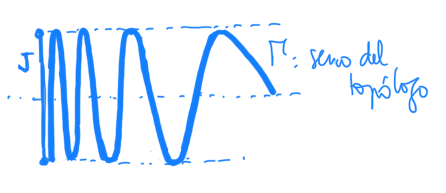
\includegraphics[scale=0.3]{images/seno_topologo} 
        \end{center}
    \end{enumerate}
\end{ej}

\section{Tabla de comportamiento}%
\label{sec:tabla_de_comportamiento_conx}
%TODO: Fix tabla
\begin{center}    
\begin{tabular}{c | c | c | c | c |}
& Subespacios & Cocientes & Productos & Sumas\\
\hline\\
    Conexión & $\times$ & \checkmark & \checkmark & $\times$\\
    \hline\\
               & $\{0, 1\} \subset \left[ 0, 1 \right]$ & Mantra $3$ & Pivote & Cada sum. ab. y cerr.\\
    \hline\\
\end{tabular}
\end{center}

\begin{prop}
$X \times Y$ conexo $\Leftrightarrow X$ y $Y$ conexo.
\end{prop} 
\begin{demo}
$\Rightarrow)$ Mantra $3$ para las proyecciones.

$\Leftarrow)$ Fijamos $a \in X$.
\begin{gather*}    
\forall y \in Y,
\begin{rcases}
    Z_y = \underbrace{\left( X \times \{y\} \right)}_{\approx X}\cup \underbrace{\left( \{a\} \times Y \right)}_{\approx Y} \text{ dos conx. se cortan en } \left( a, y \right) \xRightarrow{\text{Piv.}} Z_y \text{ conx.}\\
    \bigcap_{y \in Y} Z_y = \{a\} \times Y \neq \emptyset
\end{rcases} \xRightarrow{\text{Piv.}} \\
\bigcup_{y \in Y} Z_y = X \times Y \text{ conx.} 
\end{gather*}
%TODO: Imagen
\begin{center}
    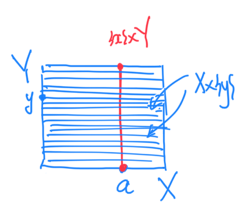
\includegraphics[scale=0.3]{images/dem_conx2_conx} 
\end{center}
\end{demo}


\chapter{Componentes conexas y conexión local}%
\label{cha:componentes_conexas_y_conexion_local}
\section{Componentes}%
\label{sec:componentes}
\begin{defi}
Una \underline{componente conexa} (c.c) de $X$ es un subespacio conexo maximal.
\end{defi}

\begin{prop}
\begin{enumerate}
    \item $\forall a \in X.\ C\left( a \right) = \bigcup_{a \in A \text{conx.}} A$ es conexo (pivote), $a \in C\left( a \right)$.
    \item $E \subset X$ conexo: 
    \[
    C\left( a \right) \cap E \neq \emptyset \Rightarrow C\left( a \right) \cup E \text{ conx. (pivote)} \Rightarrow C\left( a \right) \cup E \text{ es uno de los } A \text{ de } C\left( a \right) \Rightarrow E \subset C\left( a \right) 
    \]
    Luego, 
    \begin{itemize}
        \item $C\left( a \right)$ maximal $\Rightarrow$ componente conexa.
        \item $a \neq b: C\left( a \right) = C\left( b \right)$ ó $C\left( a \right) \cap C\left( b \right) = \emptyset$ [Usar $E = C\left( b \right)$]
    \end{itemize}

    \item $\overline{C\left( a \right)}$ conexo (mantra adh.) $\Rightarrow \overline{C\left( a \right)} = \underbrace{C\left( a \right)}_{\text{cerr.}}$ (maximalidad)
    %TODO: Fix
    \item[1. + 2. + 3.] $\Rightarrow X = \bigsqcup_{C \stackrel{\text{c.c}}{\subset}  X} C$ es una \underline{partición} en cerrados disjuntos.
\end{enumerate} 
\end{prop}

\begin{ej}
\begin{enumerate}
    \item $X_{\text{discreto}}: C\left( x \right) = \{x\}$ (puntos abiertos y cerrados)
    \item $\mathbb{Q}_u : C\left( p \right) = \{p\}$ (todo intervalo de $\mathbb{R}$ tiene racionales)
    \item $\left( \mathbb{R}, \mathcal{T}_{[, )} \right): C\left( t \right) = \{t\}$ ($\mathbb{R} = \left( \leftarrow, a \right) \cup \left[ a, \rightarrow \right)$ abierto y cerrado)
    \item $X = \{0, Y_k,\ k \ge 1\} : \begin{cases}
        C\left( 0 \right) = \{0\} \text{ cerrado, no abierto} \left( \{\frac{1}{k}: k\ge 1 \}  \text{ no cerr.}\right)\\
        C\left( \frac{1}{k} \right) = \{\frac{1}{k}\} \text{ cerrado y abierto.} 
    \end{cases} $
\end{enumerate}
\end{ej}

\begin{defi}
Un espacio cuyas componentes son los puntos se llama \underline{totalmente disconexo}. 
\end{defi}

\begin{prop}
Las componentes conexas de $X \times Y$ son los puntos de componentes conexas.
\end{prop}
\begin{demo}
$C \subset \underbrace{X}_{\xrightarrow{p} X} \times \underbrace{Y}_{\xrightarrow{q} Y} \Rightarrow p\left( C \right)$ y $q\left( C \right)$ conexos (imagen continua) $\Rightarrow \begin{cases}
    p\left( C \right) \subset E \stackrel{\text{c.c}}{\subset}  X\\
    q\left( C \right) \subset F \stackrel{\text{c.c}}{\subset}  Y
\end{cases} \Rightarrow C \subset E \times F \xRightarrow{\text{Max. de} C} C = E\times F$.
\end{demo}

\section{Conexión local}%
\label{sec:conexion_local}
\begin{defi}
$X$ es \underline{localmente conexo}  si $\forall x \in X,\ \exists \mathcal{B}^x$ base de entornos abiertos conexos.
\end{defi}

\begin{prop}
$X$ es localmente conexo $\Leftrightarrow$ la componente conexa de un abierto es abierta.
\end{prop}
\begin{demo}
\begin{itemize}
    \item $\Rightarrow)$ Si $x \in C \cerr U \ab X \Rightarrow \exists \underbrace{U^x}_{\text{ab. conx.}} \subset U \Rightarrow U^x \subset C \Rightarrow C \stackrel{\text{ab.}}{X}$.
    \item $\Leftarrow)\ \mathcal{B}^x = \{C\left( x \right) \stackrel{\text{c.c}}{\subset} U \ab X : x \in U\}$. Con $C\left( x \right)$ abierto por ser c.c de abierto.
\end{itemize}
\end{demo}

\underline{Ejercicio}: $X$ es localmente conexo $\Leftrightarrow \forall x \in X,\ \exists \mathcal{V}^x$ base de entornos conexos.

\begin{ej}[Esencial]
$\{0, \frac{1}{k} : k \ge 1\} = Y \subset \mathbb{R}_u$ \underline{no} es localmente conexo. 
\begin{demo}
    La $\text{c.c}\left( 0 \right) = \{0\}$ no es abierto. Directamente:
    \begin{align*}
        0 \in \underbrace{V}_{\text{ent. de } 0 \in \mathbb{R}} \cap Y &\Rightarrow V \supset \left( 0, \varepsilon \right),\ \exists 0 < \underbrace{\theta}_{\not\in \mathbb{Q}} < \frac{1}{k} < \varepsilon < 1\\
        &\Rightarrow V\cap Y \subset \underbrace{\left( \leftarrow, \theta \right)}_{\ni 0} \cup \underbrace{\left( \theta, \rightarrow \right)}_{\ni \frac{1}{k}}  \Rightarrow V \cap Y \text{ no conexo.} 
    .\end{align*}
\end{demo}
\end{ej}

\underline{Ejercicio}:
\begin{enumerate}
    \item Analizar una sucesión de segmentos que convergen a otro:
    \begin{center}
        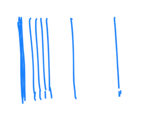
\includegraphics[scale=0.3]{images/suc_conv_otro} 
    \end{center}
    \item ¿Y el seno del topólogo?
\end{enumerate}

\section{Tabla de comportamiento}%
\label{sec:tabla_de_comportamiento_loc_conx}
%TODO: Fix tabla
\begin{center}    
\begin{tabular}{c | c | c | c | c |}
& Subespacios & Cocientes & Productos & Sumas\\
\hline\\
    Conexión local & $\times$ & \checkmark & \checkmark & $\times$\\
    \hline\\
               & Ejemplo esencial & No banal & Prod. ent. conx. & Suma como sum's\\
    \hline\\
\end{tabular}
\end{center}


\begin{prop}
Sea $f : X \rightarrow Y$ identificación con $X$ localmente conexo $\Rightarrow Y$ es localmente conexo.
\end{prop}
\begin{demo}
    El diagrama siguiente resume el argumento (si se lee en el orden adecuado).
    \begin{center}
        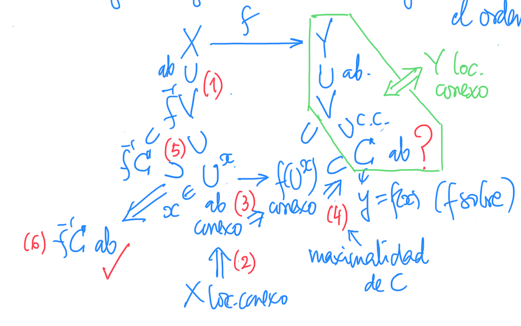
\includegraphics[scale=0.3]{images/dem_loc_conx_loc_conx} 
    \end{center}
\end{demo}
